\documentclass[11pt]{article}
\usepackage[a4paper,margin=27mm]{geometry}
\usepackage[T1]{fontenc}
\usepackage{lmodern,microtype,amsmath,amssymb,amsthm,mathtools,enumitem,comment}
\usepackage{tikz}
\usepackage{xcolor}
\newcommand{\chg}[1]{{\color{red}#1}}
\newcommand{\chgb}[1]{{\color{red}#1}}
\newenvironment{chgblockb}{\color{red}}{}
\usepackage{comment}
\usetikzlibrary{arrows.meta,calc}
\usepackage[most]{tcolorbox}
\usepackage[font=small,labelfont=bf]{caption}
\usepackage[colorlinks=true,linkcolor=blue,citecolor=blue,urlcolor=blue]{hyperref}



\colorlet{wone}{blue!70!black}
\colorlet{wtwo}{orange!85!black}
\colorlet{wthree}{green!50!black}
\colorlet{aone}{blue!22}
\colorlet{atwo}{orange!32}
\colorlet{athree}{green!22}

\newtcolorbox{stmt}[1]{enhanced,breakable,colback=white,colframe=black!55,boxrule=0.5pt,arc=1pt,
  left=5pt,right=5pt,top=3pt,bottom=3pt,fonttitle=\bfseries\small,coltitle=black,colbacktitle=black!8,title={#1}}
\DeclareRobustCommand{\stp}[1]{\tikz[baseline=(n.base)]\node[circle,draw,inner sep=0.7pt,minimum size=11pt,font=\scriptsize\bfseries](n){#1};}
\newenvironment{steps}{\begin{enumerate}[label=\stp{\arabic*},leftmargin=*,itemsep=2pt]}{\end{enumerate}}



\hypersetup{pdftitle={Coherence and Dominance under General Rankings}}

\newtheorem{theorem}{Theorem}[section]
\newtheorem{lemma}[theorem]{Lemma}
\newtheorem{proposition}[theorem]{Proposition}
\newtheorem{corollary}[theorem]{Corollary}
\theoremstyle{definition}
\newtheorem{definition}[theorem]{Definition}
\newtheorem{example}[theorem]{Example}
\theoremstyle{remark}
\newtheorem{remark}[theorem]{Remark}

\newcommand{\F}{\mathcal F}
\newcommand{\G}{\mathcal G}
\newcommand{\M}{\mathcal M}
\newcommand{\C}{\mathcal C}
\newcommand{\U}{\mathcal U}
\newcommand{\Lf}{\mathfrak L}
\newcommand{\supp}{\operatorname{supp}}
\newcommand{\cl}{\operatorname{cl}}
\setlist{itemsep=1pt,topsep=3pt}

\title{Dominance Generalised}
\author{Jason Konek}
\date{}

\begin{document}
\maketitle

\begin{abstract}
Here's a pretty little abstract. It's such a pretty little abstract. It does everything you want an abstract to do. It's a real eye-catcher. And it lets the reader know just what they're in for.

\end{abstract}




\section{Introduction}\label{sec:intro}


Dominance arguments are commonly used to justify the claim that some axioms or other are requirements of rationality. For example, De~Finetti argued that an agent's forecasts or estimates of bounded random variables ought to be probabilistic expectations \cite[\S1.6, \S3.3]{deFinetti1974}. This is necessary and sufficient for any finite collection of those estimates to avoid uniform dominance when evaluated using a loss function known as the Brier score. A finite set of estimates is uniformly dominated if there is some alternative set of forecasts/estimates that is guaranteed to get a smaller penalty (according to the loss function). Dominance seems to indicate a structural defect along whatever dimension of evaluation the loss function tracks. If the Brier score tracks a dimension of evaluation that is of cardinal importance to rationality, then forecasts/estimates that are dominated are plausibly rationally impermissible. Hence non-probabilistic estimates are rationally impermissible. Probabilistic estimates, in contrast, are rationally permissible (or at least they pass every test the dominance argument considers).


A number of authors have provided dominance arguments for coherence norms like probabilism~\cite{Joyce2009,Predd2009,SSK2009,Pettigrew2022,Nielsen2023}, norms governing updating like conditionalization~\cite{Briggs2020,Nielsen2021}, and deference norms like the Principal Principle~\cite[Chapter~10]{Pettigrew2016}. As elegant and insightful as these arguments are, they also muddle together some things that we really ought to keep distinct. De~Finetti's argument uses the Brier score. The arguments mentioned just above use a family of loss functions known as \textit{proper scoring rules}. They also assume a range of technical constraints, \textit{e.g.}, additivity, continuity, etc. (exactly which assumptions are in play vary from argument to argument). The various axioms on loss functions play two different roles. Firstly, they are meant to justify the claim that the loss function tracks a dimension of evaluation that is of cardinal importance to rationality. For example, most arguments listed here assume that loss function are \textit{truth-directed}, in the sense that moving an agent's estimates uniformly closer to the truth decreases the penalty that they receive. This seems non-negotiable if the loss function is to count as a measure of \textit{accuracy}. And facts about accuracy plausibly explain facts about epistemic rationality. Secondly, the ``core'' axioms (meant to capture the type of evaluation in play) together with the ``merely technical'' axioms jointly ensure that the loss functions in question have the structure needed for the dominance argument to work.

These two different roles should be kept separate. It is important to have a clear sense of whether there is some common structure that drives all (or most) extant variants of dominance arguments, and if so, what it is. That way, we can clearly distinguish which axioms on loss functions (i) only serve to pin down a relevant dimension of evaluation, (ii) which do this and also supply some requisite structure, necessary for the argument to run (and what structure they supply), and (iii) which are merely structural or technical axioms. Indeed, we should really apply this thought to every modelling choice that goes into the dominance argument. The choice to use real-valued loss functions, for example, to penalise performance along a given dimension of evaluation imports a lot of structure (it makes comparisons complete/total, transitive, Archimedean, etc.). Sorting out which assumptions are playing which roles is necessary to fully understand what is going on in any given argument. It is also important for providing new dominance arguments in new settings. For example, to provide a dominance argument for coherence axioms on \textit{imprecise} probability models, we need to know what structure would be required to run such an argument. We then need to identify either loss functions or more general loss ``rankings'' that track an important dimension of evaluation and (perhaps supplemented with technical axioms) supply the requisite structure. If we take axioms (\textit{e.g.}, propriety) from one setting (\textit{e.g.}, probabilism) and assume that we must impose a similar axiom in another setting (\textit{e.g.}, coherence for lower previsions or sets of desirable gambles) without clearly delineating what role(s) they were actually playing in the original argument, we might be mislead into thinking that the task is impossible.


To that end, we will present dominance arguments in what we take to be their most general form. We will not assume anything whatsoever about how to model an agent's state of opinion, what makes such a state coherent, or how to evaluate those states. The aim is to identify the minimal structure needed to run a dominance argument.



\section{Framework}\label{sec:framework}

Let $\Omega$ be a nonempty set of \emph{worlds}. Let $\M$ be a non-empty set of models. We will not assume anything about what sorts of models live in $\M$. $\M$ could be a set of precise credence functions, or Dempster-Shafer belief functions, or comparative belief relations, or lower previsions, or partial preference relations, or sets of desirable gambles, or choice/rejection functions, or probability filters, or whatever else you like. Indeed, there is no need to think of the elements of $\M$ as uncertainty models \textit{per se}, or even \textit{models} at all. $\M$ is just an unstructured set of options or things---perhaps ice cream cones, or holiday packages, etc. But our target application is uncertainty models. So we will continue to talk about $\M$ as a set of uncertainty models.




A \emph{ranking} $L=(\preceq_\omega)_{\omega\in\Omega}$ is a family of binary relations on $\M$, one for each $\omega\in\Omega$. These relations measure how well a model performs at a given task in a world. We say that $c\preceq_\omega m$ just in case $c$ performs at least as well as $m$ at $\omega$. For example, if $\M$ is a set of decision models which make recommendations about how to choose, then $c\preceq_\omega m$ might reflect the fact that $c$ does a better job guiding choice than $m$ at $\omega$. We will not assume anything about what sort of task is at issue, or what dimension(s) of evaluation these relations reflect. For general $\M$ (ice cream cones, holiday packages, etc.), the relations $\preceq_\omega$ just capture some way in which the options are better or worse at a world $\omega$.

The asymmetric part of a relation $\preceq_\omega$ is given by
\[
c\prec_\omega m\quad:\Longleftrightarrow\quad c\preceq_\omega m\ \text{and not}\ m\preceq_\omega c .
\]
Models $c$ and $m$ are \emph{equivalent} if $c\preceq_\omega m$ and $m\preceq_\omega c$ for every $\omega$. At the outset, we do not assume anything about these relations (completeness, transitivity, reflexivity, etc.).

For any ranking $L$ and any models $c,m\in\M$, we say that $c$ \emph{dominates} $m$ if
\[
(\forall\omega\in\Omega)\ c\preceq_\omega m\qquad\text{and}\qquad(\exists\omega\in\Omega)\ m\not\preceq_\omega c .
\]
We say that $m$ is \emph{undominated under $L$} if no $c\in\M$ dominates it. $\U_L$ is the set of models in $\M$ undominated under $L$.

Let $\Lf$ be a putatively complete class of reasonable rankings. It contains all and only the reasonable rankings of models in $\M$. In what follows, we will make a few minimal assumptions about this class. Firstly, we assume that there is some nonempty set $\C\subseteq\M$ of ``coherent'' models that are ``not obviously suboptimal'' at the relevant task. We do not assume anything substantive about coherence. It is just a special status that a model can have. Any model that is not coherent is incoherent. 


Secondly, we assume that each ranking recognises this special status by treating them as \textit{undominated}, at least for some privileged subset of coherent models. More carefully, for each reasonable ranking $L\in\mathfrak L$,  we assume that there is a nonempty, maximal class of coherent models, $\C_L\subseteq\C$, which is undominated under $L$.
\begin{enumerate}[label=\textbf{(LA)},leftmargin=*]
\item \textbf{Local admissibility.} $\C_L\coloneqq \C\cap\U_L\neq\varnothing$.
\end{enumerate}

Thirdly, the rankings $L\in\mathfrak L$ collectively render \textit{all} coherent models undominated.
\begin{enumerate}[label=\textbf{(CA)},leftmargin=*]
\item \textbf{Coherent admissibility.} $\C=\bigcup_{L\in\mathfrak L}\C_L$.
\end{enumerate}

Now choose a reasonable ranking $L\in\mathfrak L$. By local admissibility (LA), $L$ renders some privileged subset of coherent models, $\C_L$, undominated. By coherent admissibility (CA), every coherent model is rendered undominated by some such ranking. But (LA) does \textit{not} rule out the possibility that additional, incoherent models are undominated as well. That is, we do not simply \textit{assume} that incoherent models are defective, in the sense of being dominated relative to all reasonable rankings. The job of the dominance argument below is to \textit{prove} this stronger claim given one additional assumption.





\section{Fan-KKM theorem}\label{sec:kkm}

The general dominance argument is a trivial application of a seminal result by Fan and Knaster--Kuratowski--Mazurkiewicz \cite[Theorem~17.46]{AliprantisBorder2006}.







%Fan's extension applies to arbitrary sets of worlds \cite[Theorem~17.46]{AliprantisBorder2006}.

\begin{theorem}[Fan--KKM]\label{thm:fan-kkm}
Let $D$ be a nonempty subset of a Hausdorff topological vector space $V$. Suppose $\Psi$ assigns to each $d\in D$ a closed subset $\Psi(d)\subseteq V$, at least one of which is compact, and for every finite nonempty $F\subseteq D$,
\[
\operatorname{conv}F\subseteq\bigcup_{d\in F}\Psi(d).
\]
Then $\bigcap_{d\in D}\Psi(d)$ is nonempty and compact.
\end{theorem}


To get a feel for what theorem~\ref{thm:fan-kkm} says, consider a three world sample space $\Omega=\{\omega_1,\omega_2,\omega_3\}$. Let $V=\mathbb R^{\Omega}$ be the set of all real-valued functions $f:\Omega\rightarrow\mathbb R$ equipped with the product topology. This is a Hausdorff topological vector space. Let $D\coloneqq\{\delta_{\omega_i}:\omega_i\in\Omega\}$ be the set of indicator functions $\delta_{\omega_i}$ which put probability 1 on $\omega_i$ and probability 0 on all other worlds. Then $\operatorname{conv}D$ is $\Delta_\Omega$, the set of probability mass functions on $\Omega$. We can picture $\Delta_\Omega$ as a triangle plot. Finally, let $\Psi(\delta_{\omega_i})=A_{\omega_i}$. The sets $A_{\omega_1}$, $A_{\omega_2}$ and $A_{\omega_3}$ are each closed (and compact) sets of probability mass functions. Given these choices of $V$, $D$ and $\Psi$, the condition that for every finite nonempty $F\subseteq D$,
\[
\operatorname{conv}F\subseteq\bigcup_{d\in F}\Psi(d):=\bigcup_{\delta_{\omega_i}\in F}A_{\omega_i},
\]
is equivalent to saying that each probability mass function $p\in\Delta_\Omega$ lies in a set $A_{\omega_i}$ which is such that $p$ assigns positive mass to $\omega_i$. For example, $\delta_1$ lies in $A_{\omega_1}$ and also assigns probability 1 to $\omega_1$. Theorem~\ref{thm:fan-kkm} then guarantees there is some probability mass function $p^*$ that lies in the intersection of these three sets.



\begin{figure}[ht]
\centering
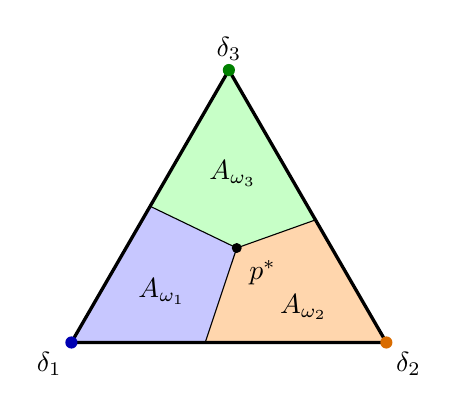
\begin{tikzpicture}
\begin{scope}[xshift=6cm]
 \coordinate (d1) at (0,0); \coordinate (d2) at (4,0); \coordinate (d3) at (2,3.46);
 \coordinate (e12) at (1.7,0); \coordinate (e23) at (3.1,1.557); \coordinate (e13) at (1,1.73);
 \coordinate (c) at (2.1,1.2);
 \fill[aone] (d1)--(e12)--(c)--(e13)--cycle;
 \fill[atwo] (d2)--(e23)--(c)--(e12)--cycle;
 \fill[athree] (d3)--(e13)--(c)--(e23)--cycle;
 \draw[very thick] (d1)--(d2)--(d3)--cycle;
 \draw (e12)--(c) (e23)--(c) (e13)--(c);
 \fill[wone] (d1) circle (2.2pt); \fill[wtwo] (d2) circle (2.2pt); \fill[wthree] (d3) circle (2.2pt);
 \node[below left] at (d1) {$\delta_1$};
 \node[below right] at (d2) {$\delta_2$};
 \node[above] at (d3) {$\delta_3$};
 \node at (1.15,0.65) {$A_{\omega_1}$};
 \node at (2.95,0.45) {$A_{\omega_2}$};
 \node at (2.05,2.15) {$A_{\omega_3}$};
 \fill (c) circle (1.8pt) node[below right=1pt] {$p^*$};
\end{scope}
\end{tikzpicture}
\caption{\chg{The Fan--KKM covering condition on a three-world simplex.}}
\label{fig:kkm}
\end{figure}




In this little example, $\Omega$ is finite. But in general $\Omega$ is an arbitrary (possibly infinite) set of worlds. To apply theorem~\ref{thm:fan-kkm} in this more general setting, we will let $V=\mathbb R^{2^\Omega}$ be the set of all real-valued functions $f:2^\Omega\rightarrow\mathbb R$ on the power set of $\Omega$, $2^\Omega$, once again equipped with the product topology. This too is a Hausdorff topological vector space. And we will let $D\coloneqq\{\delta_{\omega_i}:\omega_i\in\Omega\}$ be the set of finitely additive probability functions $\delta_{\omega_i}$ which put probability 1 on $\{\omega_i\}$ and probability 0 on any other singleton. \chg{Then $\operatorname{conv}D$ is the set of finitely supported probabilities, a subset of the set $\Delta$ of all finitely additive probabilities.}



\begin{definition}\label{def:finitely-additive-probability}
A map $p:2^\Omega\to[0,1]$ is a \emph{finitely additive probability function} iff:
\begin{enumerate}[label=\textup{(FA\arabic*)}]
  \item $p(\Omega)=1$;
  \item $p(E)\geq p(\varnothing)$;
  \item if $E\cap F=\varnothing$, then $p(E\cup F)=p(E)+p(F)$.
\end{enumerate}
\end{definition}


\chg{Equip $\Delta$ with the subspace topology inherited from $V=\mathbb R^{2^\Omega}$. It is a closed subset of $[0,1]^{2^\Omega}$, since (FA1)--(FA3) are equalities and inequalities between finitely many coordinates. Thus $\Delta$ is compact by Tychonoff's theorem and closed in the Hausdorff space $V$.}

Let $p_\omega\coloneqq p(\{\omega\})$ and $\supp p\coloneqq\{\omega:p_\omega>0\}$.  $p$ is \emph{finitely supported} if $p(F)=1$ for some finite $F\subseteq\Omega$. Finitely additive probabilities need not be countably additive, finitely supported, and indeed need not give positive probability to any world.





\section{The general dominance argument}\label{sec:gen-dom}

\begin{definition}\label{def:selection}\label{def:selection-data}
Let $L\in\mathfrak L$ be a ranking and $m\in\M$ be a model. A \textit{KKM-selection} for $m$ is a map $s^m:\Delta\to\M$ which selects a model $s^m(p)$ for each probability $p\in\Delta$ and a family of closed subsets $(A^m_\omega)_{\omega\in\Omega}$ of $\Delta$ such that:
\begin{enumerate}[label=(S\arabic*),leftmargin=3em]
\item\label{S1} for every $\omega\in\Omega$ and every $p\in A^m_\omega$ we have $s^m(p)\preceq_\omega m$;
\item\label{S2} for every finitely supported $p\in\Delta$ there is $\omega\in\Omega$ with $p_\omega>0$ and $p\in A^m_\omega$;
\item\label{S3} for every $p\in\bigcap_{\omega\in\Omega}A^m_\omega$ there is $\omega\in\Omega$ with $m\not\preceq_\omega s^m(p)$.
\end{enumerate}
\end{definition}

In what follows, we drop the superscripts and treat KKM-selections as pairs involving a map $s:\Delta\to\M$ and family $(A_\omega)_{\omega\in\Omega}$. But bear in mind that KKM-selections may vary from model to model. 


\begin{theorem}\label{thm:selection}
Let $\Omega$ be any nonempty set, $L$ any ranking and $m\in\M$. If $s$ and $(A_\omega)_{\omega\in\Omega}$ form a KKM-selection for $m$, then $\bigcap_\omega A_\omega\ne\varnothing$, and $s(p)$ dominates $m$ for every $p\in\bigcap_\omega A_\omega$.
\end{theorem}
\begin{proof}
Let $V\coloneqq\mathbb R^{2^\Omega}$, $D\coloneqq\{\delta_\omega:\omega\in\Omega\}$ and $\Psi(\delta_\omega)\coloneqq A_\omega$. Each $A_\omega$ is a closed subset of the compact space $\Delta$ and hence is itself compact \chg{and closed in $V$}. For every finite nonempty $F\subseteq\Omega$, $\operatorname{conv}\{\delta_\omega:\omega\in F\}=\{p\in\Delta:p(F)=1\}$. Condition \ref{S2} ensures that for each $p\in\Delta$ with $p(F)=1$, there is some $\omega\in F$ with $p_\omega>0$ and $p\in A_\omega$. This entails
\[
\operatorname{conv}\{\delta_\omega:\omega\in F\}
\subseteq\bigcup_{\omega\in F}A_\omega.
\]
Theorem~\ref{thm:fan-kkm} therefore gives us $\bigcap_\omega A_\omega\ne\varnothing$. For every $p$ in this intersection, \ref{S1} and \ref{S3} imply that $s(p)$ dominates $m$.
\end{proof}



Theorem~\ref{thm:selection} is the heart of the general dominance argument. To complete it, we need a \textit{dominance principle} connecting the rational status of a model with facts about dominance. We assume:
\begin{enumerate}[label=\textbf{(D)},leftmargin=*]
\item\label{principle:dominance} \textbf{Dominance.} A model $m\in\M$ is
\begin{align*}
&\text{\emph{rationally permissible} (relative to $\Lf$)}&&\text{\chg{iff} }(\exists L\in\Lf)\ m\in\U_L;\\
&\text{\emph{irrational} (relative to $\Lf$)}&&\text{\chg{iff} }(\forall L\in\Lf)\ m\notin\U_L.
\end{align*}
\end{enumerate}
That is, a model is rationally permissible if there is \textit{some} reasonable way of measuring performance which makes it come out undominated. It is irrational if \textit{every} reasonable way of measuring performance makes it come out dominated.




%This says that it is irrational to use a model $m$ for a given purpose or task if on \textit{any} reasonable way of measuring good performance at that task (any $L\in\mathfrak L$), there is some alternative $m_L^\prime$ that dominates it, in the sense that it could not possibly do worse and might do better (according to $L$); moreover the alternative does not itself suffer this defect (it is undominated, \textit{i.e.}, $m_L^\prime\in\U_L$). On the flip side, it is rationally permissible to use a model for a purpose if there is \textit{some} reasonable way of measuring good performance that renders $m$ free of the defect of domination. Of course, some particular evaluator (a single forecaster or decision-maker, a governmental organisation, etc.) might care about some ways of measuring good performance and not others. In that case, we must tailor $\mathfrak L$ appropriately.



With this dominance principle in hand, we can provide a general recipe for how to argue that all coherent models are rationally permissible and all incoherent models are irrational.
\begin{enumerate}[label=\textbf{(P\arabic*)},leftmargin=*]
\item $\Lf$ satisfies (LA), (CA) and
\begin{enumerate}
\item[(S)]\label{condition:selection} for every $L\in\Lf$ and every incoherent $m\in\M\setminus\C$, there is a KKM-selection for $m$.
\end{enumerate}
\item \textbf{Dominance} (D).
\item Theorem~\ref{thm:selection}.
\item[\textbf{(C)}]\label{conclusion:complete-class} The rationally permissible models are exactly the coherent models, and the irrational models are exactly the incoherent models.
\end{enumerate}

\chg{The inference to (C) uses (CA), (S) and (D); it does not require (LA).}




A few remarks are in order before we argue that this is the common core that drives all (or most) extant variants of dominance arguments. Firstly, nothing in Definition~\ref{def:selection} guarantees that the selected models $s(p)$ are undominated. So the dominator that Theorem~\ref{thm:selection} produces may itself be dominated. If our selection maps always yield models $s(p)$ that are undominated, then Theorem~\ref{thm:selection} yields the following corollary.



\begin{corollary}\label{cor:undominated-dominators}
Let $s$ and $(A_\omega)_{\omega\in\Omega}$ be a KKM-selection for $m$, and suppose $s(p)\in\U_L$ for every $p\in\Delta$. Then $m$ has an undominated dominator.
\end{corollary}
\begin{proof}
\chg{By Theorem~\ref{thm:selection}, some $s(p)$ dominates $m$; by hypothesis, $s(p)\in\U_L$.}
\end{proof}

Secondly, it is worth noting that \ref{S3} holds automatically for any KKM selection which satisfies the following strengthening of \ref{S1}:
\begin{enumerate}[label=(S\arabic*$^\prime$),leftmargin=3em]
\item\label{S1'} for every $\omega\in\Omega$ and every $p\in A_\omega$ we have $s(p)\prec_\omega m$.
\end{enumerate}
\noindent Similarly, \ref{S3} holds if no selected model $s(p)$ is equivalent to $m$.


Finally, \chg{Definition~\ref{def:selection}} allows KKM-selections to vary from model to model. But many extant dominance argument do not make use of this flexibility. They establish that there is a single selection map $s:\Delta\to\M$ such that every incoherent model has a KKM-selection with that same fixed selection map $s$. A generalisation of this \emph{fixed selection} approach allows a countable sequence $(s^j)_{j\in\mathbb N}$ of such selection maps such that every incoherent model has a KKM-selection with selection map $s^j$ for some $j$.









\section{Applications to accuracy}\label{sec:applications}

For a bounded function $g:\Omega\to\mathbb R$, define $E_pg$ first on simple functions by
\[
E_p\Bigl(\sum_{i=1}^n a_i\mathbf1_{E_i}\Bigr)
\coloneqq\sum_{i=1}^n a_i p(E_i),
\]
where $(E_i)_{i=1}^n$ partitions $\Omega$, and then extend by uniform approximation.

\begin{lemma}\label{lem:prob}
For each $p\in\Delta$, expectation is linear and monotone, with $E_p\mathbf1_\Omega=1$ and $|E_pg|\le\|g\|_\infty$. For every bounded $g$, the map $p\mapsto E_pg$ is affine and continuous on $\Delta$. If $p(F)=1$ for a finite $F$, then $E_pg=\sum_{\omega\in F}p_\omega g(\omega)$.
\end{lemma}
\begin{proof}
Finite additivity makes the definition on simple functions independent of the partition and gives linearity, monotonicity and the norm bound. The bound ensures a unique extension under uniform approximation, preserving these properties. For simple $g$, $p\mapsto E_pg$ is a finite linear combination of coordinate maps and is therefore affine and continuous. For simple $g_n\to g$ uniformly, $|E_pg_n-E_pg|\le\|g_n-g\|_\infty$ uniformly in $p$, so the same holds for bounded $g$. The finite-support identity holds first for simple functions and then by uniform approximation.
\end{proof}

For the numerical applications, a ranking is given by a \emph{loss} $\ell:\chg{\M}\times\Omega\to[0,\infty]$, with $m\preceq_\omega m'$ iff $\ell(m,\omega)\le\ell(m',\omega)$. A function $f$ from a topological space to $[0,\infty]$ is \emph{lower semicontinuous} if $\{z:f(z)\le a\}$ is closed for every real $a$. For finite $\Omega$ write $E_p\ell(m,\cdot)\coloneqq\sum_\omega p_\omega\ell(m,\omega)$ with $0\cdot\infty=0$.

\begin{lemma}[KKM-selections for losses]\label{lem:loss-one-stage}
Let $L$ be given by a loss $\ell$, and let $p\mapsto s(p)$ be a map $\Delta\to\chg{\M}$ such that:
\begin{enumerate}[label=(\roman*)]
\item for every $\omega$, $p\mapsto\ell(s(p),\omega)$ is lower semicontinuous on $\Delta$;
\item for every $m\in\chg{\M}$ and every finitely supported $p$, some $\omega$ with $p_\omega>0$ has $\ell(s(p),\omega)\le\ell(m,\omega)$.
\end{enumerate}
Let $m\in\chg{\M}$ and put $A_\omega\coloneqq\{p\in\Delta:\ell(s(p),\omega)\le\ell(m,\omega)\}$. Then \ref{S1} and \ref{S2} hold. If no $s(p)$ is tied at every world with $m$, then \ref{S3} holds, and some $s(p)$ dominates $m$.
\end{lemma}
\begin{proof}
$A_\omega$ is closed by (i), and equals $\Delta$ if $\ell(m,\omega)=\infty$. \ref{S1} is the definition of $A_\omega$, and \ref{S2} is (ii) for this $m$. \chg{At a common point, $s(p)$ is at least as good as $m$ at every world; the absence of a tie therefore gives \ref{S3}.} Apply Theorem~\ref{thm:selection}.
\end{proof}

\chg{In each numerical application below, the complete-class conclusion is (C) in \S\ref{sec:gen-dom}, under (D), for the one-ranking family $\Lf=\{L\}$: (S) follows from Lemma~\ref{lem:loss-one-stage}\chgb{ (in \S\ref{sec:probabilism}, from Proposition~\ref{prop:probabilism})}, and (LA) and (CA) follow from the stated protection argument.}

The protection argument covers every candidate. In Propositions~\ref{prop:proper}, \ref{prop:updating} and~\ref{prop:chance}\chgb{ and Corollary~\ref{cor:probabilism}}, each candidate $s(p)$ is coherent and is proved to be undominated. In Proposition~\ref{prop:updating} this is proved directly for every coherent strategy; it is not derived from Bayes optimality under the probability $q$ used for coverage. So $s(p)\in\C\cap\U_L$ for every $p\in\Delta$. By Corollary~\ref{cor:undominated-dominators}, in each of these numerical applications every incoherent model is dominated by a coherent model that is itself undominated, namely $s(p)$ for any $p\in\bigcap_\omega A_\omega$.

\subsection{Proper losses on finitely many worlds}

\begin{proposition}[{\cite{Predd2009,Pettigrew2022}}]\label{prop:proper}
Let $\Omega$ be finite, let $\ell$ be a loss on $\chg{\M}$, and let $p\mapsto s(p)$ map $\Delta$ onto $\C\subseteq\chg{\M}$. Suppose each $s(p)$ is the unique Bayes model for $p$, that is, $E_p\ell(s(p),\cdot)<E_p\ell(m,\cdot)$ for every $m\ne s(p)$, and $p\mapsto\ell(s(p),\omega)$ is lower semicontinuous for every $\omega$. Then every incoherent model is dominated by some $s(p)$, every coherent model is undominated, and $\{L\}$ satisfies \chg{(S), (LA) and (CA)}.
\end{proposition}
\begin{proof}
If $\chg{\M}$ is a singleton $\{c\}$, then $c$ is coherent and there is nothing to prove. Otherwise $E_p\ell(s(p),\cdot)<\infty$ for every $p$, since $E_p\ell(s(p),\cdot)<E_p\ell(m,\cdot)$ for some $m$.

\emph{Weak dominators of $s(p)$.} If $m\preceq_\omega s(p)$ for every $\omega$, then $E_p\ell(m,\cdot)\le E_p\ell(s(p),\cdot)$, so $m=s(p)$ by uniqueness. Hence no model dominates $s(p)$, which gives \chg{(CA)} since the map is onto $\C$. Hence also no $s(p)$ is tied at every world with an incoherent model, since such a model would weakly dominate $s(p)$.

\emph{Coverage.} Let $m\in\chg{\M}$ and $p\in\Delta$ (every $p$ is finitely supported). If $\ell(s(p),\omega)>\ell(m,\omega)$ for every $\omega\in\supp p$, then, as $E_p\ell(s(p),\cdot)$ is finite, $E_p\ell(m,\cdot)<E_p\ell(s(p),\cdot)$, contradicting Bayes optimality. This is Lemma~\ref{lem:loss-one-stage}(ii), and (i) is assumed. For incoherent $m$, Lemma~\ref{lem:loss-one-stage} gives a KKM-selection; this is \chg{(S)}.
\end{proof}

\subsection{Probabilism on arbitrary domains}\label{sec:probabilism}

\begin{chgblockb}
Let $\Omega$ be any nonempty set, $\M=[0,1]^{2^\Omega}$ with the product topology, and $\C\coloneqq\Delta$. Consider the following conditions on a ranking $L=(\preceq_\omega)_{\omega\in\Omega}$ on $\M$.
\begin{description}[leftmargin=1.5em,font=\normalfont\bfseries]
\item[(CC) Closed comparisons.] For every $m\in\M$ and $\omega\in\Omega$, the set $B_\omega(m)\coloneqq\{p\in\Delta:p\preceq_\omega m\}$ is closed in $\Delta$.
\item[(SA) Support coverage.] For every finitely supported $p\in\Delta$ and every $m\in\M$ there is $\omega\in\supp p$ with $p\preceq_\omega m$.
\item[(N) No incoherent ties.] There are no $m\in\M\setminus\Delta$ and $p\in\Delta$ such that $p\preceq_\omega m$ and $m\preceq_\omega p$ for every $\omega\in\Omega$.
\end{description}
(CC) is the qualitative counterpart of lower semicontinuity. It requires closedness only as the probability varies with the rival $m$ held fixed; it does not require the relations $\preceq_\omega$ to be closed in $\M\times\M$. If the relations are incomplete, (SA) is stronger than the requirement that no rival be strictly better than $p$ at every world in $\supp p$, since a rival may be incomparable with $p$ at some of those worlds. The proof below uses (SA) as displayed.

\begin{proposition}\label{prop:probabilism}
Let $L$ satisfy (CC), (SA) and (N). Then every $m\in\M\setminus\Delta$ is dominated under $L$ by a member of $\Delta$. If every member of $\Delta$ is undominated under $L$, this dominator is undominated.
\end{proposition}
\begin{proof}
Fix $m\notin\Delta$. Put $s(p)\coloneqq p$ and $A_\omega\coloneqq B_\omega(m)$. These sets are closed by (CC). \ref{S1} holds by the definition of $A_\omega$, and \ref{S2} is (SA). At a point $p\in\bigcap_\omega A_\omega$ we have $p\preceq_\omega m$ for every $\omega$, so (N) gives some $\omega$ with $m\not\preceq_\omega p$; this is \ref{S3}. Apply Theorem~\ref{thm:selection}, and Corollary~\ref{cor:undominated-dominators} for the second claim.
\end{proof}

For any family $\Lf$ of rankings satisfying (CC), (SA) and (N), Proposition~\ref{prop:probabilism} gives (S). With (CA) and (D), it therefore yields the complete-class conclusion (C). Here (CA) requires each probability to be undominated under some ranking, not under every ranking.

\emph{Truth-directedness.} For $m\in\M$, $E\subseteq\Omega$ and $\omega\in\Omega$ put $e_\omega(m,E)\coloneqq|m(E)-\mathbf 1_E(\omega)|$. The ranking $L$ is \emph{truth-directed} if, for every $\omega\in\Omega$ and $m,n\in\M$:
\begin{enumerate}[label=(TD\arabic*),leftmargin=3em]
\item\label{TD1} if $e_\omega(m,E)\le e_\omega(n,E)$ for every $E$, then $m\preceq_\omega n$;
\item\label{TD2} if, moreover, $e_\omega(m,E)<e_\omega(n,E)$ for some $E$, then $m\prec_\omega n$.
\end{enumerate}
Truth-directedness characterises these rankings as evaluations of accuracy; the dominance proof uses only (CC), (SA) and (N). The following construction shows that these requirements are jointly consistent with protection of every probability.

\begin{proposition}[Existence]\label{prop:accuracy-existence}
For every nonempty $\Omega$, there is a truth-directed ranking satisfying (CC), (SA) and (N) under which every member of $\Delta$ is undominated. Its singleton family therefore satisfies (LA) and (CA).
\end{proposition}
\begin{proof}
Write $m\unlhd_\omega n$ if $e_\omega(m,E)\le e_\omega(n,E)$ for every $E\subseteq\Omega$. We extend these comparisons in two ways.

First, for $p\in\Delta$ put
\[
J(p,\omega)\coloneqq 1-2p_\omega+\sum_{\nu\in\Omega}p_\nu^2,
\]
where a sum of nonnegative terms is the supremum of its finite subsums. Since $\sum_\nu p_\nu\le1$, $J$ takes values in $[0,2]$ and is lower semicontinuous in $p$. The function $\nu\mapsto p_\nu$ is the uniform limit of its finite truncations, so Lemma~\ref{lem:prob} gives $E_q[\nu\mapsto p_\nu]=\sum_\nu q_\nu p_\nu$. Consequently, for $p,q\in\Delta$,
\begin{equation}\label{eq:atomic-brier}
E_qJ(p,\cdot)-E_qJ(q,\cdot)
=\sum_{\nu\in\Omega}(p_\nu-q_\nu)^2.
\end{equation}
If $p\unlhd_\omega q$ and $p\ne q$, then $p_\omega>q_\omega$. Indeed, otherwise equality holds at $\{\omega\}$, and the inequalities $p(E)\le q(E)$ for $E\subseteq\Omega\setminus\{\omega\}$, applied also to their complements within that set, force $p=q$. Moreover $p_\nu\le q_\nu$ for $\nu\ne\omega$. Thus
\[
J(p,\omega)=(1-p_\omega)^2+\sum_{\nu\ne\omega}p_\nu^2
<J(q,\omega).
\]

Second, for each $n\notin\Delta$, compactness of $\Delta$ in the product topology supplies a finite set of events $\mathcal E_n$ such that
\[
d_n\coloneqq\min_{q\in\Delta}\sum_{E\in\mathcal E_n}(n(E)-q(E))^2>0.
\]
To see this, take a basic open neighbourhood of $n$ disjoint from $\Delta$; its finite set of coordinates has a compact projection of $\Delta$ not containing the corresponding projection of $n$. Put
\[
H_n(m,\omega)\coloneqq\sum_{E\in\mathcal E_n}e_\omega(m,E)^2.
\]
The finite Brier identity gives, for every $p\in\Delta$,
\begin{equation}\label{eq:finite-witness-brier}
E_p\bigl[H_n(n,\cdot)-H_n(p,\cdot)\bigr]
=\sum_{E\in\mathcal E_n}(n(E)-p(E))^2\ge d_n.
\end{equation}

Define $m\preceq_\omega n$ iff at least one of the following holds:
\begin{enumerate}[label=(\roman*),leftmargin=3em]
\item $m\unlhd_\omega n$;
\item $m,n\in\Delta$ and $J(m,\omega)\le J(n,\omega)$;
\item $m\in\Delta$, $n\notin\Delta$ and $H_n(n,\omega)-H_n(m,\omega)\ge d_n$.
\end{enumerate}
\emph{Truth-directedness.} Clause (i) gives \ref{TD1}. If $m\unlhd_\omega n$ strictly on some event, clause (i) cannot hold in reverse. Neither can (ii), by the strict inequality for $J$ above, or (iii), since $H_m(m,\omega)\le H_m(n,\omega)$ whenever that reverse clause applies. Thus \ref{TD2} holds.

\emph{(CC).} For $n\in\Delta$, $B_\omega(n)=\{p\in\Delta:J(p,\omega)\le J(n,\omega)\}$, a closed set. For $n\notin\Delta$, it is the union of the closed sets $\{p\in\Delta:p\unlhd_\omega n\}$ and $\{p\in\Delta:H_n(n,\omega)-H_n(p,\omega)\ge d_n\}$.

\emph{(SA).} If $p$ is finitely supported and $n\in\Delta$, \eqref{eq:atomic-brier} gives $E_pJ(p,\cdot)\le E_pJ(n,\cdot)$, so $J(p,\omega)\le J(n,\omega)$ at some $\omega\in\supp p$. When $n\notin\Delta$, \eqref{eq:finite-witness-brier} ensures $H_n(n,\omega)-H_n(p,\omega)\ge d_n$ at some such $\omega$.

\emph{Protection and (N).} If $m\notin\Delta$ were weakly better than $q\in\Delta$ at every world, only clause (i) could apply. On any nonempty proper event $E$, worlds inside and outside $E$ would give $m(E)\ge q(E)$ and $m(E)\le q(E)$ respectively; on $\varnothing$ and $\Omega$, $q$ is already correct. Hence $m=q$, a contradiction. This also proves (N). If instead $p\in\Delta$ is weakly better than $q$ everywhere, then $J(p,\omega)\le J(q,\omega)$ everywhere. Taking $q$-expectations in \eqref{eq:atomic-brier} gives $p_\nu=q_\nu$ for every $\nu$, so $J(p,\omega)=J(q,\omega)$ everywhere. Clause (ii) then gives the reverse comparisons at every world, excluding dominance. Finally $\Delta\ne\varnothing$, so the singleton family satisfies (LA) and (CA).
\end{proof}

Consequently, the family of all truth-directed rankings satisfying (CC), (SA), (N) and (LA) satisfies (CA). Under (D), its rationally permissible models are exactly the finitely additive probabilities. The auxiliary Brier comparisons in the existence proof are not additional axioms on this family.

\emph{A numerical corollary.} For $q\in\Delta$ and $f:\Omega\to[0,\infty]$ put $E_qf\coloneqq\sup_{k\in\mathbb N}E_q(f\wedge k)$. Applying Lemma~\ref{lem:prob} to $f\wedge k$ and taking increasing limits gives, with $0\cdot\infty=0$,
\begin{gather*}
E_{ap+(1-a)q}f=aE_pf+(1-a)E_qf\quad(0<a<1),\\
p(F)=1,\ F\text{ finite}\ \Longrightarrow\ E_pf=\textstyle\sum_{\omega\in F}p_\omega f(\omega),
\end{gather*}
and $f\le f'$ implies $E_qf\le E_qf'$. A loss $\ell:\M\times\Omega\to[0,\infty]$ is \emph{quasi-strictly proper} if $E_q\ell(q,\cdot)\le E_q\ell(m,\cdot)$ for all $q\in\Delta$ and $m\in\M$, strictly whenever $m\notin\Delta$.

\begin{corollary}\label{cor:probabilism}
Let $L$ be given by a quasi-strictly proper loss $\ell$ such that each $q\mapsto\ell(q,\omega)$ is lower semicontinuous on $\Delta$. Then $L$ satisfies (CC), (SA) and (N), and every member of $\Delta$ is undominated. Hence every incoherent model is dominated by a member of $\Delta$ that is itself undominated, and $\{L\}$ satisfies (S), (LA) and (CA).
\end{corollary}
\begin{proof}
\emph{Finiteness.} For $q\in\Delta$, $E_q\ell(q,\cdot)<E_q\ell(m_0,\cdot)\le\infty$ for the incoherent $m_0\equiv0$, so $E_q\ell(q,\cdot)<\infty$.

\emph{(CC).} $B_\omega(m)=\{p\in\Delta:\ell(p,\omega)\le\ell(m,\omega)\}$ is closed by lower semicontinuity, and equals $\Delta$ if $\ell(m,\omega)=\infty$.

\emph{(SA).} Let $p(F)=1$ for a finite $F$, and $m\in\M$. Then $E_p\ell(p,\cdot)=\sum_{\omega\in F}p_\omega\ell(p,\omega)<\infty$, so $\ell(p,\omega)<\infty$ for $\omega\in\supp p$. If $\ell(p,\omega)>\ell(m,\omega)$ for every $\omega\in\supp p$, then $E_p\ell(m,\cdot)=\sum_{\omega\in\supp p}p_\omega\ell(m,\omega)<E_p\ell(p,\cdot)$, contradicting propriety.

\emph{(N).} If an incoherent $m$ were tied at every world with $q\in\Delta$, then $E_q\ell(m,\cdot)=E_q\ell(q,\cdot)$, contradicting strict propriety against incoherent models.

\emph{Protection.} Suppose $m$ dominates $q\in\Delta$, with $\ell(m,w)<\ell(q,w)$; in particular $\ell(m,w)<\infty$. Weak dominance and monotonicity give $E_q\ell(m,\cdot)\le E_q\ell(q,\cdot)$, and propriety gives equality, so $E_q\ell(m,\cdot)=E_q\ell(q,\cdot)<\infty$. For $k\ge2$ put $q_k\coloneqq(1-1/k)q+\delta_w/k\in\Delta$. Propriety at $q_k$ and at $q$ gives
\[
\tfrac1k\ell(q_k,w)+(1-\tfrac1k)E_q\ell(q,\cdot)\le E_{q_k}\ell(q_k,\cdot)\le E_{q_k}\ell(m,\cdot)=\tfrac1k\ell(m,w)+(1-\tfrac1k)E_q\ell(q,\cdot).
\]
Subtracting the finite common term gives $\ell(q_k,w)\le\ell(m,w)$ for every $k$. Since $q_k\to q$ in $\Delta$, lower semicontinuity gives $\ell(q,w)\le\ell(m,w)$, a contradiction.

The remaining claims follow from Proposition~\ref{prop:probabilism}; (LA) holds because $\Delta\ne\varnothing$.
\end{proof}

Nielsen's Theorems~1--2~\cite{Nielsen2023} assume quasi-strict propriety, continuity on $\Delta$ of $q\mapsto E_p\ell(q,\cdot)$ for every $p\in\Delta$, and boundedness of $\ell(p,\cdot)$ for each $p\in\Delta$. Taking $p=\delta_\omega$ shows that his continuity assumption implies ours. Corollary~\ref{cor:probabilism} therefore obtains his protection conclusion under weaker regularity assumptions, but its exclusion conclusion is weaker: Nielsen obtains strict improvement at every world. Proposition~\ref{prop:probabilism} isolates the qualitative conditions used for selection, without numerical losses or expected-loss comparisons. Truth-directedness is a separate accuracy constraint, not one of Nielsen's admissibility conditions.

\begin{remark}[Numerical representation]\label{rem:numerical-TD}
Let $\Omega$ be infinite and $\omega\in\Omega$. No function $\ell(\cdot,\omega):\M\to[0,\infty]$ satisfies \ref{TD1} and \ref{TD2} with $m\preceq_\omega n$ read as $\ell(m,\omega)\le\ell(n,\omega)$. Indeed, $2^\Omega$ has at least the cardinality of $\mathbb R$; fix an injection $r\mapsto E_r$ from $(0,1)$ into $2^\Omega$. For $r\in(0,1)$ choose $a_r,b_r\in\M$ with errors in $\{0,1\}$: $e_\omega(a_r,E)=0$ iff $E=E_t$ for some $t<r$, and $e_\omega(b_r,E)=0$ iff $E=E_t$ for some $t\le r$. By \ref{TD2}, $\ell(b_r,\omega)<\ell(a_r,\omega)$; by \ref{TD1}, $\ell(a_s,\omega)\le\ell(b_r,\omega)$ whenever $r<s$. The intervals $(\ell(b_r,\omega),\ell(a_r,\omega))$, $r\in(0,1)$, would therefore be pairwise disjoint and each contain a distinct rational, which is impossible.

So a real-valued loss can be truth-directed only in a weakened sense. One weakening keeps \ref{TD1} and requires strict improvement only when every proposition improves: $\ell(m,\omega)<\ell(n,\omega)$ whenever $e_\omega(m,E)<e_\omega(n,E)$ for every $E$. A weighted Brier loss $\ell(m,\omega)=\sum_kw_k\,e_\omega(m,E_k)^2$ on a countable family $(E_k)$ of events, with $w_k>0$ and $\sum_kw_k<\infty$, has this property. The example shows only that the weakened constraint has a real-valued representation; it does not satisfy the whole package above. For instance, it violates (N): since $2^\Omega$ is uncountable, some $E\notin\{E_k\}$, and changing a probability's value at $E$ alone gives an incoherent model (its values at $E$ and $\Omega\setminus E$ no longer sum to $1$) tied with it at every world. 
\end{remark}
\end{chgblockb}

\subsection{Conditional updating}

Let $\Omega$ be finite and $E_1,\dots,E_k$ nonempty, pairwise disjoint, with union $\Omega$. Models are strategies $(c,a_1,\dots,a_k)\in([0,1]^{2^\Omega})^{k+1}$. A strategy is \emph{coherent} if $c,a_1,\dots,a_k\in\Delta$, $a_j(E_j)=1$ and $c(A\cap E_j)=c(E_j)a_j(A)$ for every $A$ and $j$. Let $J$ be a finite loss for credence functions on $2^\Omega$ that is strictly proper (each $q\in\Delta$ uniquely minimises $c'\mapsto E_qJ(c',\cdot)$ over $[0,1]^{2^\Omega}$) and lower semicontinuous on $\Delta$ at every world. For $\alpha,\beta>0$ put
\[
\ell((c,a),\omega)\coloneqq\alpha J(c,\omega)+\beta J(a_j,\omega)\qquad(\omega\in E_j).
\]

\begin{proposition}[{\cite{Briggs2020,Nielsen2021}}]\label{prop:updating}
Every incoherent strategy is dominated by a coherent one, every coherent strategy is undominated, and $\{L\}$ satisfies \chg{(S), (LA) and (CA)}.
\end{proposition}
\begin{proof}
\emph{Weak dominators of a coherent strategy.} Let $(c,a)$ be coherent and $(c',a')$ weakly dominate it. For each $j$, $\sum_{\omega\in E_j}c_\omega J(a'_j,\omega)=c(E_j)E_{a_j}J(a'_j,\cdot)\ge c(E_j)E_{a_j}J(a_j,\cdot)$, using $c(\{\omega\})=c(E_j)a_j(\{\omega\})$ for $\omega\in E_j$. With $E_cJ(c',\cdot)\ge E_cJ(c,\cdot)$, this gives $E_c\ell((c',a'),\cdot)\ge E_c\ell((c,a),\cdot)$, while weak dominance gives $\le$. As all quantities are finite, $E_cJ(c',\cdot)=E_cJ(c,\cdot)$, so $c'=c$. Cancelling the common term $\alpha J(c,\omega)$, weak dominance gives $J(a'_j,\omega)\le J(a_j,\omega)$ for $\omega\in E_j$. Taking expectations under $a_j$, which is concentrated on $E_j$, gives $E_{a_j}J(a'_j,\cdot)\le E_{a_j}J(a_j,\cdot)$, so $a'_j=a_j$; this includes cells with $c(E_j)=0$. Hence coherent strategies are undominated, which is \chg{(CA)}, and no incoherent strategy is tied at every world with a coherent one.

\emph{Assignment.} Put $\eta\coloneqq1/(2k)$, $x_+\coloneqq\max\{x,0\}$, and fix $w_j\in\Delta$ with $w_j(E_j)=1$. For $p\in\Delta$ let $p|_{E_j}(A)\coloneqq p(A\cap E_j)$ and
\[
r_j\coloneqq\frac{p|_{E_j}+(\eta-p(E_j))_+w_j}{\max\{p(E_j),\eta\}},\qquad \lambda_j\coloneqq\frac{(p(E_j)-\eta)_+}{\sum_i(p(E_i)-\eta)_+},\qquad q\coloneqq\sum_j\lambda_jr_j .
\]
The denominator of $\lambda_j$ is positive, since otherwise $1=\sum_ip(E_i)\le k\eta=\tfrac12$. Each $r_j\in\Delta$ with $r_j(E_j)=1$; each $\lambda_j\ge0$ with $\sum_j\lambda_j=1$; so $q\in\Delta$, $q(E_j)=\lambda_j$ and $q(A\cap E_j)=\lambda_jr_j(A)$, and $s(p)\coloneqq(q,r_1,\dots,r_k)$ is coherent. If $\lambda_j>0$ then $p(E_j)>\eta$ and $r_j=p|_{E_j}/p(E_j)$; hence $\supp q\subseteq\supp p$. All these maps are continuous in $p$, since $\max\{p(E_j),\eta\}\ge\eta>0$.

\emph{Lower semicontinuity.} $p\mapsto\ell(s(p),\omega)$ is a positive combination of $J(\cdot,\omega)$, lower semicontinuous on $\Delta$, composed with continuous maps into $\Delta$, hence lower semicontinuous.

\emph{Coverage.} $s(p)$ is Bayes for $q$: for any strategy $(c',a')$, $E_qJ(c',\cdot)\ge E_qJ(q,\cdot)$, and for each $j$ with $\lambda_j>0$, $\sum_{\omega\in E_j}q_\omega J(a'_j,\omega)=\lambda_jE_{r_j}J(a'_j,\cdot)\ge\lambda_jE_{r_j}J(r_j,\cdot)$, while cells with $\lambda_j=0$ contribute nothing. If $\ell(s(p),\omega)>\ell(m,\omega)$ for every $\omega\in\supp p$, then the same holds on $\supp q$, and finiteness of $J$ gives $E_q\ell(m,\cdot)<E_q\ell(s(p),\cdot)$, a contradiction. Lemma~\ref{lem:loss-one-stage} gives \chg{(S)}.
\end{proof}

\subsection{Chance dominance}

Let $W$ be finite, $\mathcal K\subseteq\Delta_W$ nonempty, and $\Theta\coloneqq\cl(\operatorname{conv}\mathcal K)$ (Euclidean closure). Let $\chg{\M}=[0,1]^{\mathcal F}$ for a set of events $\mathcal F\subseteq2^W$, identify $\theta\in\Delta_W$ with $(\theta(A))_{A\in\mathcal F}$, and let $\C$ be the set of credences induced by members of $\Theta$. Let $I:\chg{\M}\times W\to[0,\infty)$ be such that each $\theta\in\Delta_W$ uniquely minimises $c\mapsto E_\theta I(c)\coloneqq\sum_w\theta(w)I(c,w)$ over $\chg{\M}$, and $\theta\mapsto I(\theta,w)$ is lower semicontinuous on $\Theta$. The worlds of the ranking are the members of $\mathcal K$, and $c\preceq_\kappa d$ iff $E_\kappa I(c)\le E_\kappa I(d)$, for $\kappa\in\mathcal K$ \cite[Chapter~10]{Pettigrew2016}.

\begin{proposition}\label{prop:chance}
Every credence outside $\C$ is dominated by a member of $\C$, every member of $\C$ is undominated, and $\{L\}$ satisfies \chg{(S), (LA) and (CA)}.
\end{proposition}
\begin{proof}
\emph{Weak dominators of $\theta\in\Theta$.} If $m$ weakly dominates $\theta$, the function $\kappa\mapsto E_\kappa I(m)-E_\kappa I(\theta)$ is affine and continuous on $\Delta_W$ and nonpositive on $\mathcal K$, hence on $\Theta$. At $\kappa=\theta$, unique minimisation forces $m=\theta$. This gives \chg{(CA)}, and excludes ties at every world between members of $\C$ and other credences.

\emph{Assignment.} Here $\Delta$ is the set of finitely additive probabilities on $\mathcal K$. For $p\in\Delta$ let $\bar p(w)\coloneqq E_p[\kappa\mapsto\kappa(w)]$; by Lemma~\ref{lem:prob} $p\mapsto\bar p$ is continuous. Moreover $\bar p\in\Theta$: otherwise separation of $\bar p$ from the closed convex set $\Theta$ gives $a\in\mathbb R^W$ with $\sum_wa_w\bar p(w)>\sup_{\theta\in\Theta}\sum_wa_w\theta(w)$, while linearity and the upper bound in Lemma~\ref{lem:prob} give $\sum_wa_w\bar p(w)=E_p[\kappa\mapsto\sum_wa_w\kappa(w)]\le\sup_{\kappa\in\mathcal K}\sum_wa_w\kappa(w)$. Put $s(p)\coloneqq\bar p\in\C$. For $\kappa\in\mathcal K$, $p\mapsto E_\kappa I(s(p))=\sum_w\kappa(w)I(\bar p,w)$ is a finite nonnegative combination of lower semicontinuous functions composed with a continuous map into $\Theta$, hence lower semicontinuous.

\emph{Coverage.} If $p(F)=1$ for a finite $F\subseteq\mathcal K$, then $\bar p=\sum_{\kappa\in F}p_\kappa\kappa$ and $\sum_{\kappa\in F}p_\kappa E_\kappa I(c)=E_{\bar p}I(c)$ for every $c$. If $E_\kappa I(s(p))>E_\kappa I(m)$ for every $\kappa\in\supp p$, then $E_{\bar p}I(m)<E_{\bar p}I(s(p))$, contradicting Bayes optimality of $\bar p$. Lemma~\ref{lem:loss-one-stage} gives \chg{(S)}; the set of worlds $\mathcal K$ may be infinite.
\end{proof}

\subsection{Tie exclusion is needed}

\begin{example}\label{ex:ties}
Let $\Omega=\{1,2\}$, $\chg{\M}=[0,1]^2$, $\C=\Delta$, and $\ell(x,1)=(1-x_1+x_2)^2$, $\ell(x,2)=(1+x_1-x_2)^2$. With $d\coloneqq x_1-x_2\in[-1,1]$, $\ell(x,1)$ is decreasing and $\ell(x,2)$ increasing in $d$. So models with different $d$ are incomparable, and $x$ is tied at every world with the probability $((1+d)/2,(1-d)/2)$. No model is dominated. Put $s(p)\coloneqq p$: $E_p\ell(x,\cdot)=p_1(1-d)^2+p_2(1+d)^2$ is minimised at $d=p_1-p_2$, so (ii) of Lemma~\ref{lem:loss-one-stage} holds, and (i) holds by continuity. For incoherent $x$ the candidates and sets of Lemma~\ref{lem:loss-one-stage} satisfy \ref{S1} and \ref{S2}, but \ref{S3} fails, and the conclusion of Theorem~\ref{thm:selection} fails.
\end{example}

\bibliographystyle{plain}
\bibliography{references}

\end{document}
